\chapter{Phase stability and elastic properties study of the Ti-Ta and Ti-Nb systems}

\section{Introduction}

The present chapter is aimed at studying the formation of the metastable phases $\omega$ and $\alpha"$. As shown in chapter 1 Figure \ref{Ch1-figure:tinbelasitc} and \ref{Ch1-figure:titaelastic}, the formation of the $\alpha"$ and $\omega$ phases effects the elastic properties of the implant alloy. Understanding the effect of the metastable phases and at what compositions they form will help with alloy selection and increase the likelihood of finding a suitable alloy for the load-bearing implant appliction. The stabiliy at 0 $^\circ$K of the bcc, hcp, $omega$, $alpha"$ phases is calculated and discussed for the Ti-Ta and Ti-Nb alloys using multiple structures across the entire composition range. The elastic properties of the four phases are then calculated systematically and interaction parameters are introducted using the CALPHAD method, similar to chapter 5, to be able to predict the elastic properties as a function of composition. With an understanding of how the phases effect the elastic properties, a new theoretical framework was introduced in chapter 2 in order to be able to predict the formation of the metastable phases. This chapter uses the new theoretic framework to study Ti and the Ti-Nb system in the bcc, $\omega$ and $\alpha"$ phases. The theoretic framework is used to predict the phase fractions of the metastable phases and the mixed force constants to plot the phonon density of states. In order to ensure the accuracy of the theroretic framework, neutron scattering experiments are completed on 4 different Ti-Nb compositions. The data from the experiments is used to determine the phase fractions and phonon density of states. The results from the neutron scattering are compared with the theoretical results. The determined phase fractions are used to predict the elastic properties and compared with experimental values in literature.

\section{Modeling and Calculations}

\subsection{Computational details}

In the present work the Vienna ab-initio Simulation Package (VASP) \cite{Kresse1996} was employed to calculate the ground state energy and elastic properties of the pure elements and Ti-Nb and Ti-Ta systems in the bcc, hcp, $\omega$, and $\alpha"$ phases. The ion-electron interactions were described using the projector augmented wave (PAW) \cite{Kresse1999,Blochl1994} method and based on the previous work of comparing X-C functionals (Figure \ref{Ch2-figure:PBEvsPW91}) the exchange-correlation functional of the generalized gradient approach depicted by Perdew, Burke, and Ernzerhof (PBE-GGA) was employed \cite{Perdew1996a}. The energy convergence criterion was 10$^{-6}$ eV/atomThe Brillouin zone sampling was done using the $\gamma$-centered Monkhorst-Pack scheme \cite{Monkhorst1976a}. The ground state energy of 330 structures in the bcc phase, across the entire compostition range, were calculated using 8x8x8 k-point meshes. The ground state energy of 21 structures in the hcp phase, across the entire compostition range, were calculated using 10x10x13 k-point meshes. The ground state energy of 73 structures in the $\omega$ phase, across the entire compostition range, were calculated using 13x13x7 k-point meshes. The ground state energy of 33 structures in the $\alpha"$ phase, across the entire compostition range, were calculated using 12x11x10 k-point meshes.The elastic properties were then calculated using a $\pm$0.01 magntiude of strain.

\subsection{Modeling details}

The elastic stiffness constants were modeled using the first-principles based DFT results. The modeling was completed by calculating the difference between the first-principles calculations and a linear extrapolation between pure elements. The differences were then used to fit to the interaction parameters. Due to the limitations within the PARROT module, a mathmatica script was used to fit the interaction parameters. The mathematica script is appended in appendix C. The same modeling procedure used for the bcc phase, in Chapter 5 and 6, was used in the prsent work. The first-principles results with 70 at. \% Ti or higher were weighted heavier (x6, according to the authors' practices) than the other points for the fittings. The best fit was found by comparing the fittings obtained with one interaction parameter or with two interaction parameters. The moduli values were than calculated using pycalphad and the code in appendix D and E \cite{Otis2017}.

\section{Results and discussion}

\subsection{First-principles calculations at 0 K}

The phase stability at 0 $^\circ$K is calculated as a function of composition for the Ti-Nb and Ti-Ta systems. Figure \ref{Ch7-figure:tinb0K} shows the relative energy of the bcc, hcp, $\omega$, and $\alpha"$ phases from 100 at. \% Ti to 100 at. \% Nb. The relative energies are calculated similiarliy to the enthalpy of formation in Eq. \ref{eq: hform}, the ground state energies of the pure elements in the SER state are multipled by the composition of the specific structure and then stubtracted from the ground state energy of the structure being studied. Figure \ref{Ch7-figure:titab0K} is the relative energy of the bcc, hcp, $\omega$, and $\alpha"$ phases from 100 at. \% Ti to 100 at. \% Ta. Figure \ref{Ch7-figure:tinb0K} and \ref{Ch7-figure:titab0K} are both at 0 $^\circ$K. The figures show that the bcc and hcp phases are the lowest phases in energy. This shows that the $\omega$ and $\alpha"$ phases are stabilized by entropy.

The Ti-Nb system is chosen to study more in depth due to the experimental work avaliable in the literature which mapped the martensitic transformation temperature for Ti-Nb alloys between the 20 and 30 at. \% Nb is shown in Figure \ref{Ch7-figure:titnbms} \cite{Kim2006}.  

\subsection{Elastic properties}

For the Ti-Nb system, the elastic properties are calculated as a function of composition and are plotted in Figure \ref{Ch7-figure:tinbelastic}. The calculations are shown as symbols and the results are listed in Table \ref{Ch7-table:tinbdata}. The dotted lines are the fittings that use the interaction parameters in Table \ref{Ch7-table:intpara}. The calculations show that the hcp elastic properites go from being positive at 100 at. \% Ti to negative at 100 at. \% Nb and vice versa for the bcc phase. A negative Young's modulus can indicate that the phase is not stable at that composition. From Figure \ref{Ch7-figure:tinbelastic}, it can be seen that the Young's moduli of the $\omega$ and $\alpha"$ phases are higher than the Young's moduli of the bcc phase for all the compositions. The Young's moduli of the $\omega$ and $\alpha"$ phases are also higher than the Young's moduli of the hcp phase at almost all compositions. This would explain why in Figure \ref{Ch1-figure:tinbelasitc} the experimental Young's moduli increase in value with the formation of the metastable. 

Table \ref{Ch7-table:elasexptdata} shows the phase fraction of different Ti-Nb alloy compositions that were determined experimentally and avaliable in the literature \cite{Ozaki2004,Timoshevskii2011,Friak2012,Karre2015}. Using the interaction parameters in Table \ref{Ch7-table:intpara} and the rule of mixtures described calculates the elastic modulus of the multi-phase alloy ($E_{c}$) by:

%%
\begin{equation}
\label{eq:ruleofmix}
E_{c}=x_{p1}E_{p1}+x_{p2}E_{p2}
\end{equation}
%%

\noindent where $x_{p1}$ and $x_{p2}$ are the phase fractions of phase 1 and phase 2. $E_{p1}$ and $E_{p2}$ are the elastic modulus of the alloys in phase 1 and phase 2. After using Eq. \ref{eq:ruleofmix}, the predicted Young's moduli are compared with the experimentally determined Young's moduli. The predicted Young's moduli vary by less than XX from the experimentally determined Young's moduli. Based on the comparison, it is seen that if the phase fraction of the metastable phases can be predicted than the database can be used with the rule of mixtures to accurately predict the elastic properites. 

\subsection{Neutron scattering results}

\subsubsection{Phonon density of states at 300 K}

The phonon density of states was obtained at 300 $^\circ$K for each set of samples at each Nb composition. The phonon density of states are plotted in Figure \ref{Ch7-figure:50dos20}, \ref{Ch7-figure:50dos18}, \ref{Ch7-figure:50dos12}, \ref{Ch7-figure:50dos10}. The samples at the same composition are plotted together for comparison. The phonon density of states of the slow cooled samples, that should contain the bcc and $\omega$ phases, are plotted with dashed lines and the phonon density of states of the quenced samples, that should contain the bcc and $\alpha "$ phases, are plotted with solid lines. The fact that the different samples show different phonon DOS means that the quenching versus slow cooling worked and the samples should have different phases. In order to investigate the difference of the phonon DOS further the entropy of each sample was calculated from the phonon DOS ($g(E)$):

%%
\begin{equation}
\label{eq:phononentropy}
S_{vib} = 3 k_{B} \int_{0}^{E_{max}} \left[ \left( n+1 \right) ln\left(n+1\right) -n ln\left(n\right) \right] g(E) dE
\end{equation}
%%

\noindent where $n$ is the Bose-Einstien occupation factor \cite{Budai2014}. The entropy difference between the alloys at the same compositions is plotted in \ref{Ch7-figure:ediff}. The figure shows that the entropy difference increases from 10 mol \% Nb to 20 mol \% Nb. The increase in entropy with increasing Nb content makes sense when looking at Figure \ref{Ch1-figure:tinbelasitc}. The figure and previous research shows that the $\alpha"$ and $\omega$ phases form from approximately 10 mol \% to 0.35 mol \% Nb. At 10 mol \% Nb, only a small amount of the metastable phases form which is why the experimentally determined elastic properties still line up well with the theoretically obtained elastic properites. This is supported by the lower entropy difference between the two 10 mol \% Nb alloys. However, closer to 20 mol \% Nb, Figure \ref{Ch7-figure:tinbelastic} shows that the experimental Young's moduli is higher than computationally determined Young's moduli. Research showed that the phase fractions of the metastable phase is larger at this composition than the three other compositions studied in this work. This is supported by the larger difference in entropy at 20 mol \% Nb.

\subsubsection{Diffraction patterns at 300 K}

The diffraction patterns for each alloy are plotted in Figure \ref{Ch7-figure:50diff20}, \ref{Ch7-figure:50diff18}, \ref{Ch7-figure:50diff12} \ref{Ch7-figure:50diff10}. The slow cooled samples are plotted as solid lines and the quenched samples are plotted as dashed lines. The diffraction patterns plot the Q vs. the intensity. The plots are compared with known diffraction patterns of Ti and Nb in the four phases to determine the phase fractions. The determined phase fractions of each alloy are listed in Table \ref{Ch7-table:phasefrac}. The analysis shows that the samples at XX mol \% Nb have the XXX 

With the implementation of the theoretic framework still ongoing we compared the phase fractions obtained by the neutron scattering experiments with previous experiments also shown in Table \ref{Ch7-table:elasexptdata} \cite{Ozaki2004,Timoshevskii2011,Friak2012,Karre2015}. The determined phase fractions compare well with the previously determined phase fractions. XXXX

\subsection{Partition function approach results}

The implementation of the new theoretical framework is ongoing. Due to the difficulty of implementing a new theoretic framework, we began by calculating pure Ti. The energy was mapped for Ti in the bcc, $\omega$, and hcp phases looking for the energy minima. The quasiharmonic phonon calculations will be completed on the structures at the lowest energy minima points. The 

The continued work 

\section{Conclusion}

Based on the research done up to this point, the elastic 

\newpage
\begin{longtable}[H]{ c c c c c c c c c c }
	\caption{First-principles calculations of the elastic stiffness constants in GPa for different atomic percent compositions in the $\alpha"$, bcc, hcp, and $\omega$  phases in the Ti-Nb system at 0 $^\circ$K.} 	\label{Ch7-table:tinbdata} \\
	\hline
	Ti$_{1-b}$Nb$_b$ & c$_{11}$ & c$_{12}$ & c$_{13}$ & c$_{22}$ & c$_{23}$ & c$_{33}$ & c$_{44}$ & c$_{55}$ & c$_{66}$\\
	\hline
	\endhead
	\hline
	\endfoot
	\multicolumn{10}{c}{$\alpha"$}\\
	\hline
	Ti & 198 & 69 & 84 & 197 & 84 & 189 & 40 & 40 & 63 \\		
	TiNb$_{2}$ & A & B & C & D & E & F & G & H & I \\
	TiNb$_{3}$ & 106 & 112 & 123 & 152 & 45 & 138 & 25 & 17 & 38 \\
	TiNb$_{13}$ & A & B & C & D & E & F & G & H & I \\
	TiNb$_{94}$ & 307 & 94 & 119 & 248 & 143 & 214 & 31 & -24 & 13 \\
	TiNb$_{97}$ & 293 & 88 & 115 & 232 & 124 & 284 & 59 & -58 & 8 \\
	TiNb$_{98}$ & A & B & C & D & E & F & G & H & I \\
	Nb & 306 & 88 & 125 & 240 & 135 & 284 & 47 & -69 & 9 \\
	\hline
	\multicolumn{10}{c}{bcc}\\
	\hline
	Ti & 93 & 115 & - & - & - & - & 41 & - & - \\		
	TiNb$_{2}$ & 93 & 115 & - & - & - & - & 35 & - & - \\
	TiNb$_{13}$ & 116 & 116 & - & - & - & - & 37 & - & - \\
	TiNb$_{25}$ & 140 & 116 & - & - & - & - & 34 & - & - \\
	TiNb$_{50}$ & 181 & 121 & - & - & - & - & 31 & - & - \\
	TiNb$_{75}$ & 208 & 130 & - & - & - & - & 15 & - & - \\
	TiNb$_{94}$ & 242 & 134 & - & - & - & - & 18 & - & - \\
	TiNb$_{98}$ & 242 & 134 & - & - & - & - & 18 & - & - \\
	Nb & 245 & 144 & - & - & - & - & 27 & - & - \\
	\hline
	\multicolumn{10}{c}{hcp}\\
	\hline
	Ti & 175 & 88 & 80 & - & - & 190 & 41 & - & - \\		
	TiNb$_{2}$ & A & B & C & - & - & D & E & - & - \\
	TiNb$_{13}$ & A & B & C & - & - & D & E & - & - \\
	TiNb$_{25}$ & A & B & C & - & - & D & E & - & - \\
	TiNb$_{50}$ & A & B & C & - & - & D & E & - & - \\
	TiNb$_{75}$ & A & B & C & - & - & D & E & - & - \\
	TiNb$_{94}$ & A & B & C & - & - & D & E & - & - \\
	TiNb$_{98}$ & A & B & C & - & - & D & E & - & - \\
	Nb & 24 & 18 & 11 & - & - & 25 & -6 & - & - \\
	\hline
	\multicolumn{10}{c}{$\omega$}\\
	Ti & 194 & 87 & 61 & - & - & 246 & 54 & - & - \\
	TiNb$_{2}$ & 187 & B & C & - & - & D & E & - & - \\
	TiNb$_{13}$ & A & B & C & - & - & D & E & - & - \\
	TiNb$_{94}$ & A & B & C & - & - & D & E & - & - \\
	TiNb$_{98}$ & A & B & C & - & - & D & E & - & - \\
	Nb & 243 & 181 & 110 & - & - & 212 & -55 & - & - \\
	\hline
\end{longtable}
%%%

\newpage
\begin{table}[H]
	\caption{Evaluated interaction parameters $L_0$ and $L_1$, using Eq. \ref{eq: elastic}, for the elastic stiffness constants of the bcc, hcp, $\alpha"$ and $\omega$ phases in the Ti-Nb systems.}
	\centering
	\begin{tabular}{ c c c c c c }
		\hline
		Alloy & Interaction Parameter & $\alpha"$ & bcc & hcp & $\omega$\\
		\hline
		c$_{11}$ & $L_{0}$ & A & B & C & D \\
		& $L_{1}$ & A & B & C & D \\
		c$_{12}$ & $L_{0}$ & A & B & C & D \\
		& $L_{1}$ & A & B & C & D \\
		c$_{13}$ & $L_{0}$ & A & N/A & C & D \\
		& $L_{1}$ & A & N/A & C & D \\
		c$_{22}$ & $L_{0}$ & A & N/A & N/A & N/A \\
		& $L_{1}$ & A & N/A & N/A & N/A \\
		c$_{23}$ & $L_{0}$ & A & N/A & N/A & N/A \\
		& $L_{1}$ & A & N/A & N/A & N/A \\
		c$_{33}$ & $L_{0}$ & A & N/A & C & D \\
		& $L_{1}$ & A & N/A & C & D \\
		c$_{44}$ & $L_{0}$ & A & B & C & D \\
		& $L_{1}$ & A & B & C & D \\
		c$_{55}$ & $L_{0}$ & A & N/A & N/A & N/A \\
		& $L_{1}$ & A & N/A & N/A & N/A \\
		c$_{66}$ & $L_{0}$ & A & N/A & N/A & N/A \\
		& $L_{1}$ & A & N/A & N/A & N/A \\
		\hline
	\end{tabular}
	\label{Ch7-table:intpara}
\end{table}
\clearpage
%%%

\newpage
\begin{table}[H]
	\caption{Phase fractions and experimetally determined $E$ compared with the predicted $E$ using the rule of mixtures and interaction parameters in Table \ref{Ch7-table:intpara} for the Ti-Nb system.}
	\centering
	\begin{tabular}{ c c c c c c }
		\hline
		Alloy & x(Nb) & Phase Fraction & Expt $E$ & Calc $E$ & Reference \\
		\hline
		c$_{11}$ & $L_{0}$ & A & B & C & D \\

		\hline
	\end{tabular}
	\label{Ch7-table:elasexptdata}
\end{table}
\clearpage
%%%

\newpage
\begin{table}[H]
	\caption{Phase fractions determined from the diffraction patterns for the Ti-Nb alloys.}
	\centering
	\begin{tabular}{ c c c c c c }
		\hline
		Alloy & x(Nb) & \multicolumn{4}{c}{Phase Fraction} \\
		 &  & bcc & hcp & $\omega$ & $\alpha"$ \\
		\hline
		TiNb$_{20}$ & 0.2 & A & B & C & D \\
		TiNb$_{18}$ & 0.2 & A & B & C & D \\
		TiNb$_{12}$ & 0.2 & A & B & C & D \\
		TiNb$_{10}$ & 0.2 & A & B & C & D \\
		\hline
	\end{tabular}
	\label{Ch7-table:phasefrac}
\end{table}
\clearpage
%%%


\pagebreak
\begin{figure}[H]
	\centering
	\includegraphics[width=\textwidth]{Chapter-7/Figures/tinb0k.png}
	\caption{Relative energy of the bcc, hcp, $\omega$, $\alpha"$ phases in the Ti-Nb system are plotted from 100 at. \% Ti to 100 at. \% Nb.}
	\label{Ch7-figure:tinb0K}
\end{figure}

\pagebreak
\begin{figure}[H]
	\centering
	\includegraphics[width=\textwidth]{Chapter-7/Figures/tita0k.png}
	\caption{Relative energy of the bcc, hcp, $\omega$, $\alpha"$ phases in the Ti-Ta system are plotted from 100 at. \% Ti to 100 at. \% Ta.}
	\label{Ch7-figure:titab0K}
\end{figure}

\pagebreak
\begin{figure}[H]
	\centering
	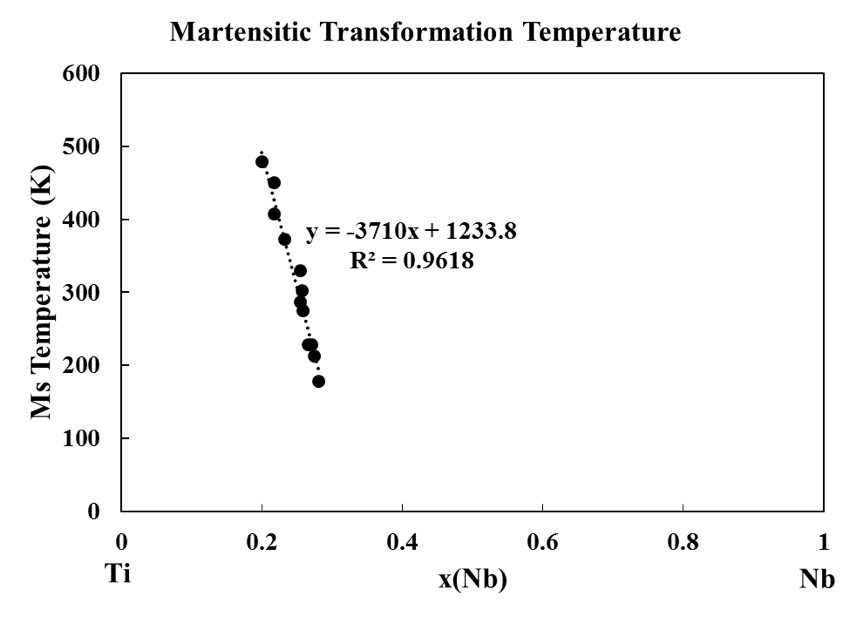
\includegraphics[width=\textwidth]{Chapter-7/Figures/tinbms.png}
	\caption{Martensitic transformation temperature is plotted versus the Ti-Nb composition.}
	\label{Ch7-figure:titnbms}
\end{figure}

\pagebreak
\begin{figure}[H]
	\centering
	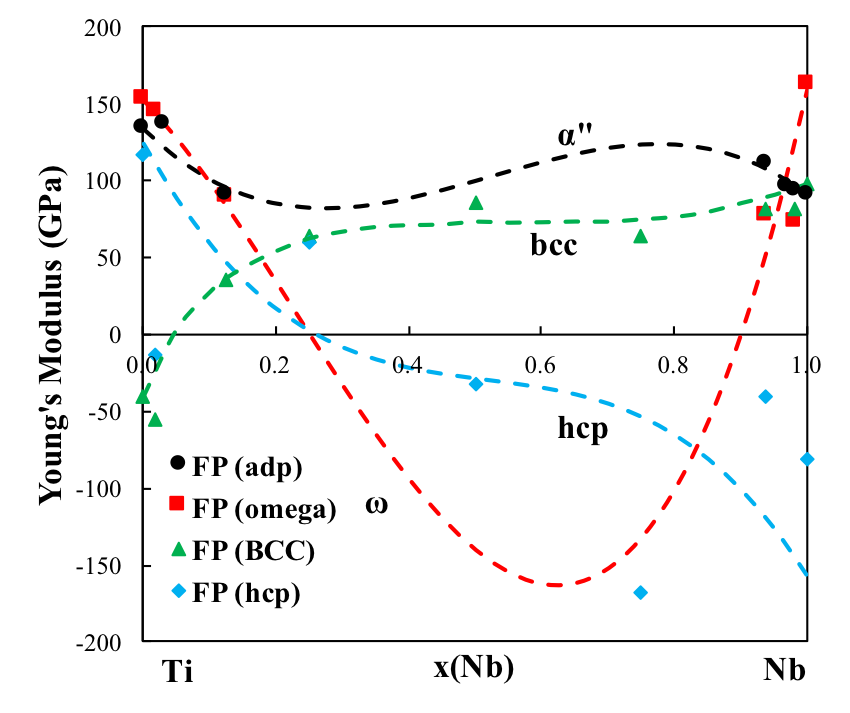
\includegraphics[width=\textwidth]{Chapter-7/Figures/tinbelastic.png}
	\caption{Eelastic properites of the bcc, hcp, $\omega$, $\alpha"$ phases in the Ti-Nb system calculated from first-principles based on DFT are plotted as symbols. The CALPHAD fitting are plotted as the dashed lines. The figure is plotted from 100 at. \% Ti to 100 at. \% Nb.}
	\label{Ch7-figure:tinbelastic}
\end{figure}

\pagebreak
\begin{figure}[H]
	\centering
	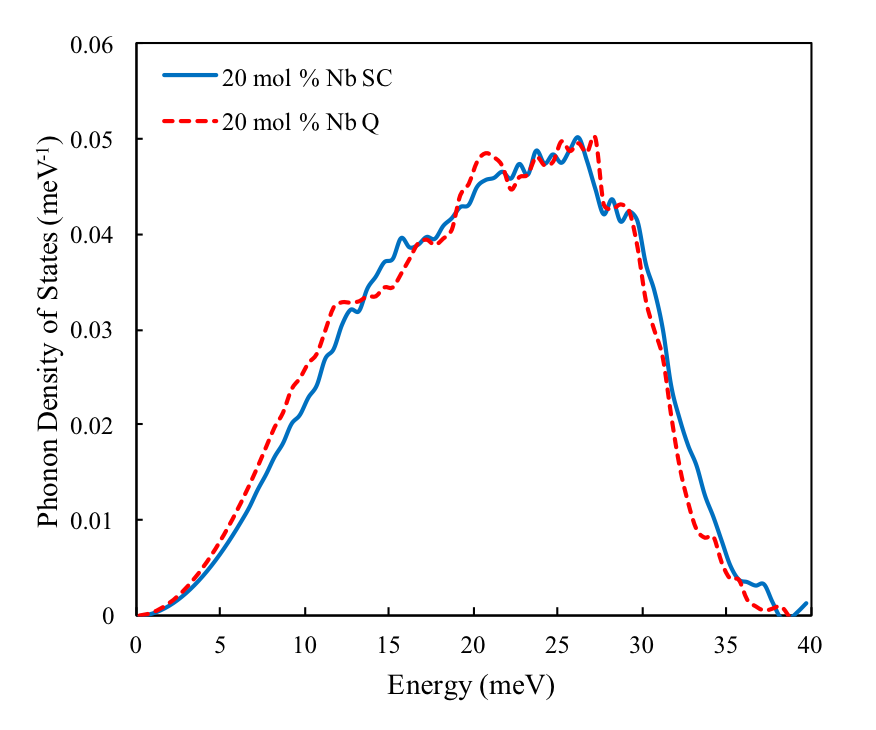
\includegraphics[width=\textwidth]{Chapter-7/Figures/50dos20.png}
	\caption{Phonon density of states is plotted for the TiNb alloy at 20 at. \% Nb. The dashed line represents the slow cooled sample while the solid line represents the quenched sample.}
	\label{Ch7-figure:50dos20}
\end{figure}

\pagebreak
\begin{figure}[H]
	\centering
	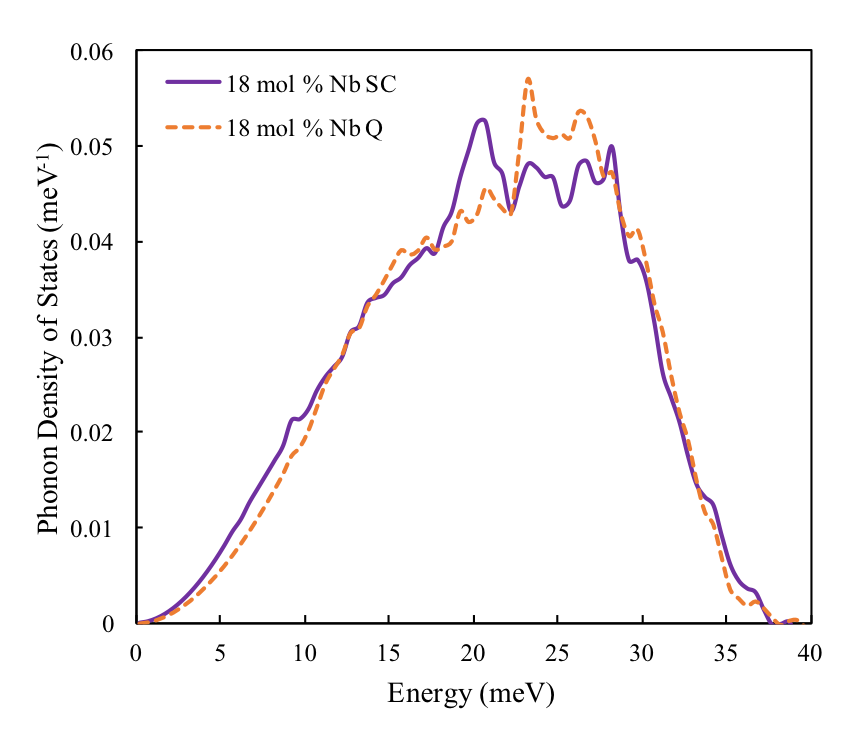
\includegraphics[width=\textwidth]{Chapter-7/Figures/50dos18.png}
	\caption{Phonon density of states is plotted for the TiNb alloy at 18 at. \% Nb. The dashed line represents the slow cooled sample while the solid line represents the quenched sample.}
	\label{Ch7-figure:50dos18}
\end{figure}

\pagebreak
\begin{figure}[H]
	\centering
	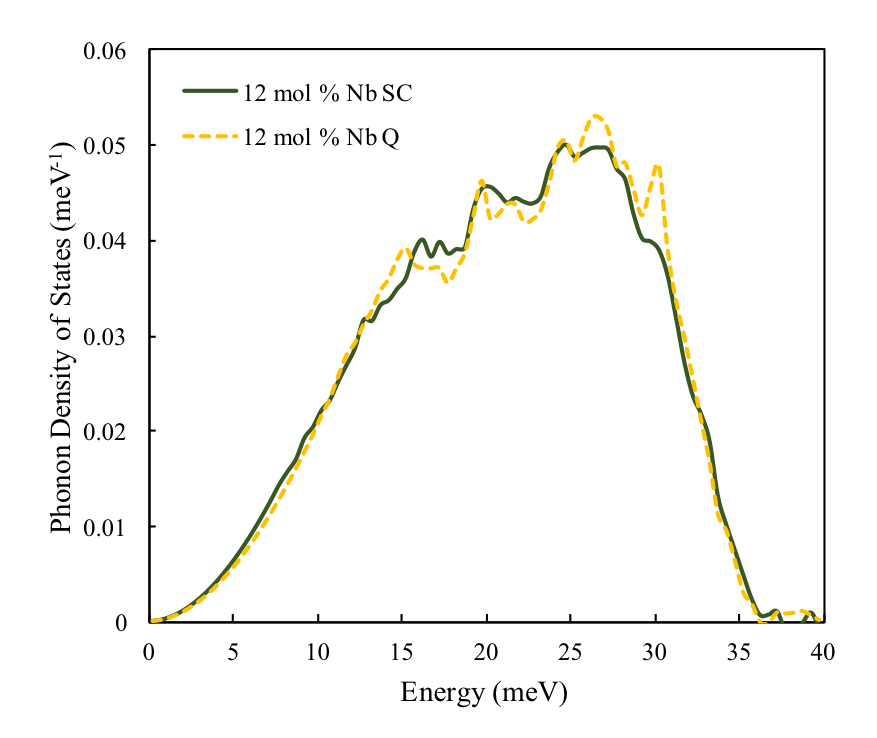
\includegraphics[width=\textwidth]{Chapter-7/Figures/50dos12.png}
	\caption{Phonon density of states is plotted for the TiNb alloy at 12 at. \% Nb. The dashed line represents the slow cooled sample while the solid line represents the quenched sample.}
	\label{Ch7-figure:50dos12}
\end{figure}

\pagebreak
\begin{figure}[H]
	\centering
	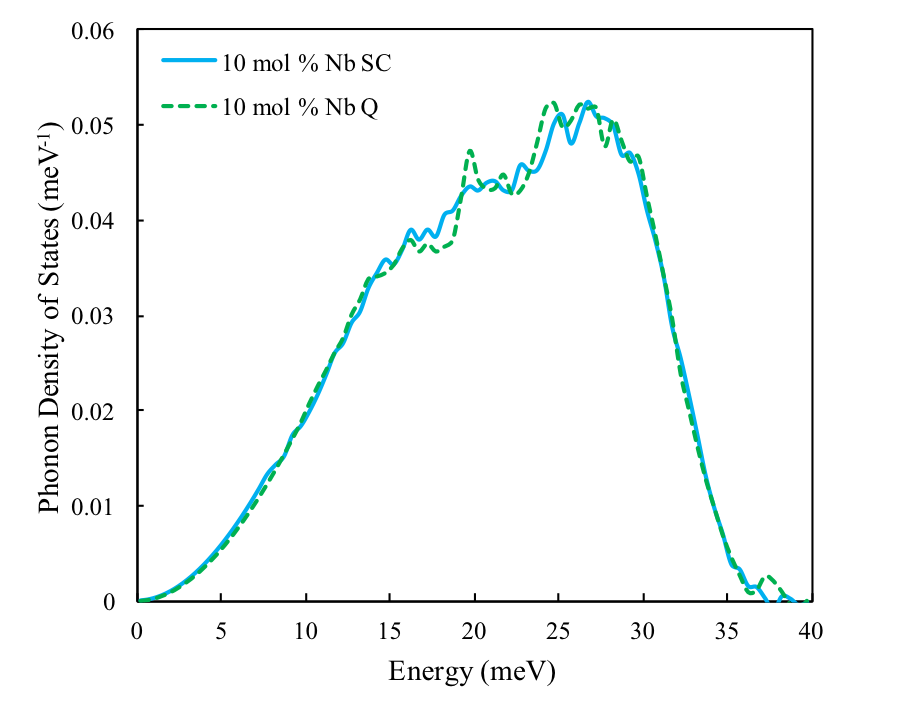
\includegraphics[width=\textwidth]{Chapter-7/Figures/50dos10.png}
	\caption{Phonon density of states is plotted for the TiNb alloy at 10 at. \% Nb. The dashed line represents the slow cooled sample while the solid line represents the quenched sample.}
	\label{Ch7-figure:50dos10}
\end{figure}

\pagebreak
\begin{figure}[H]
	\centering
	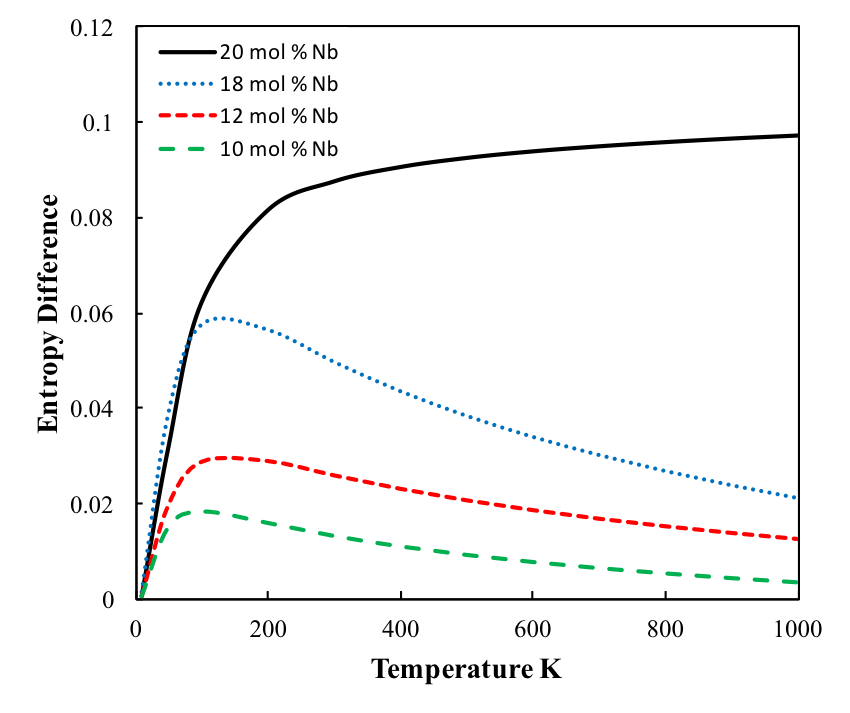
\includegraphics[width=\textwidth]{Chapter-7/Figures/ediff.png}
	\caption{Entropy difference between the Ti-Nb alloys with the same alloy composition is plotted as a function of temperature.}
	\label{Ch7-figure:ediff}
\end{figure}

\pagebreak
\begin{figure}[H]
	\centering
	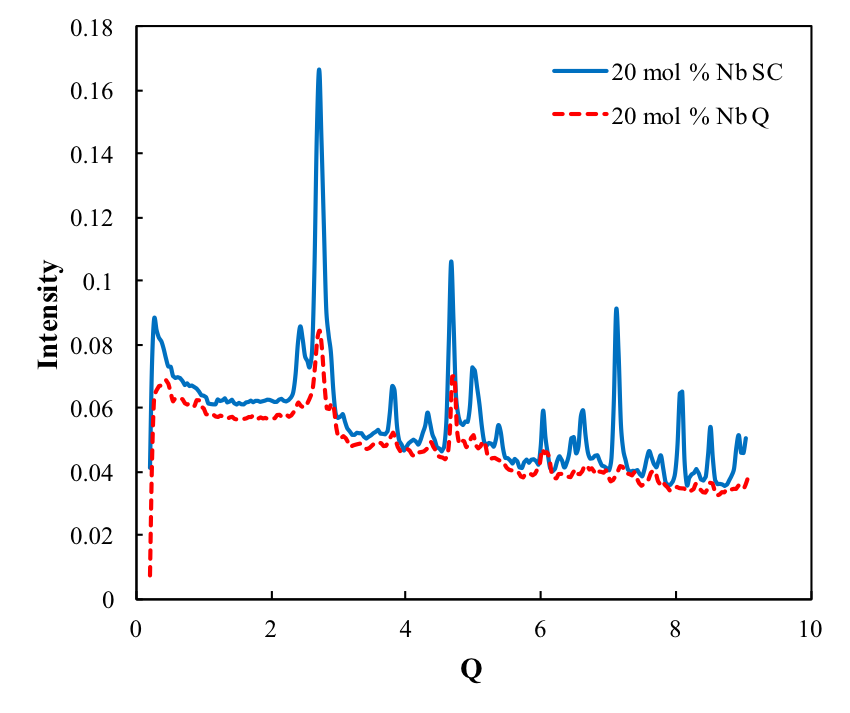
\includegraphics[width=\textwidth]{Chapter-7/Figures/50diff20.png}
	\caption{Diffraction pattern of the Ti-Nb alloy at 20 at. \% Nb. The dashed line represents the slow cooled sample while the solid line represents the quenched sample.}
	\label{Ch7-figure:50diff20}
\end{figure}

\pagebreak
\begin{figure}[H]
	\centering
	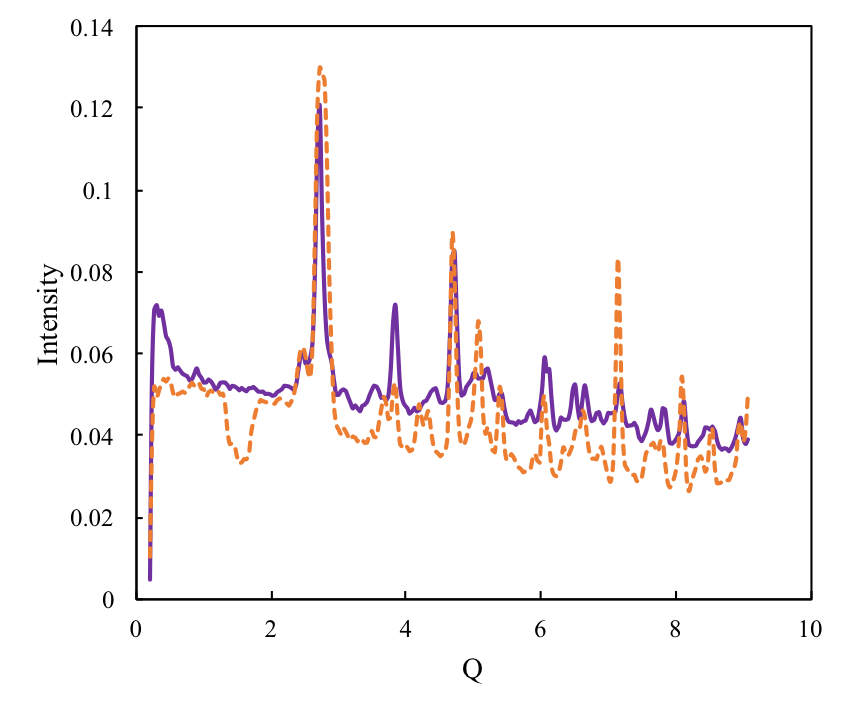
\includegraphics[width=\textwidth]{Chapter-7/Figures/50diff18.png}
	\caption{Diffraction pattern of the Ti-Nb alloy at 18 at. \% Nb. The dashed line represents the slow cooled sample while the solid line represents the quenched sample.}
	\label{Ch7-figure:50diff18}
\end{figure}

\pagebreak
\begin{figure}[H]
	\centering
	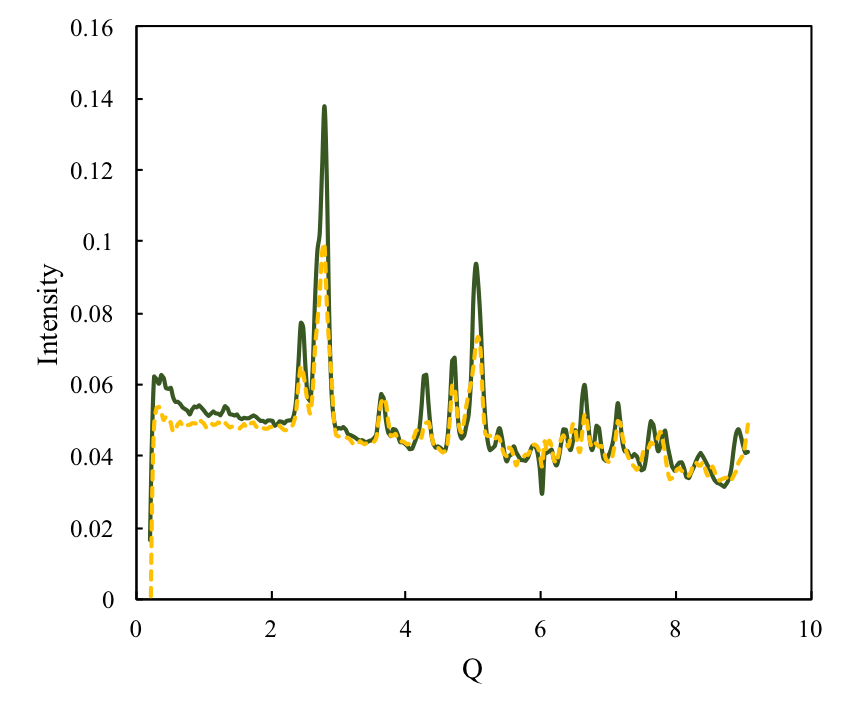
\includegraphics[width=\textwidth]{Chapter-7/Figures/50diff12.png}
	\caption{Diffraction pattern of the Ti-Nb alloy at 12 at. \% Nb. The dashed line represents the slow cooled sample while the solid line represents the quenched sample.}
	\label{Ch7-figure:50diff12}
\end{figure}

\pagebreak
\begin{figure}[H]
	\centering
	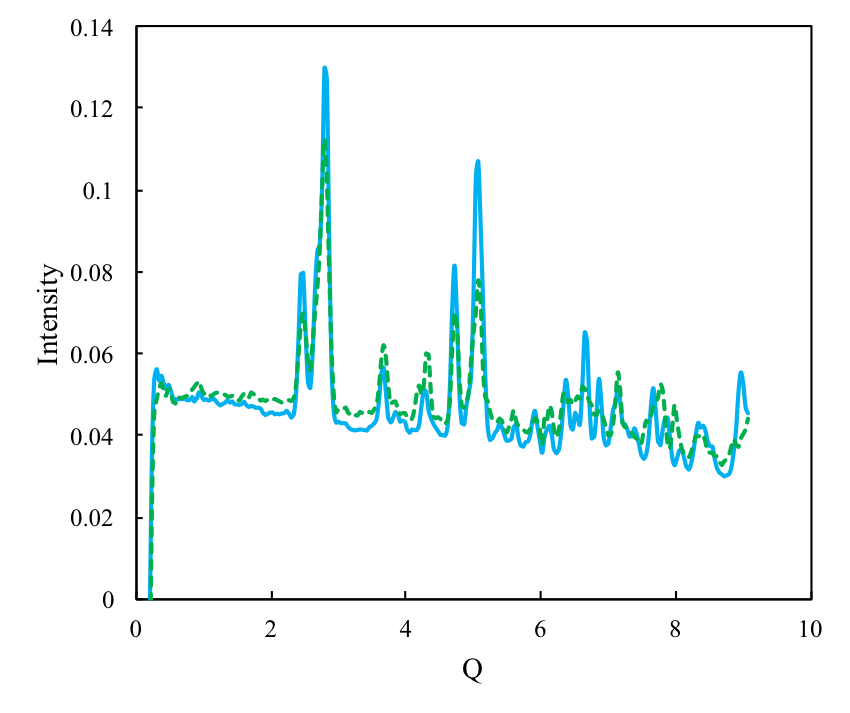
\includegraphics[width=\textwidth]{Chapter-7/Figures/50diff10.png}
	\caption{Diffraction pattern of the Ti-Nb alloy at 10 at. \% Nb. The dashed line represents the slow cooled sample while the solid line represents the quenched sample.}
	\label{Ch7-figure:50diff10}
\end{figure}
